%        File: paper_v1.tex
%     Created: Sun Mar 25 03:00 pm 2018 C
% Last Change: Sun Mar 25 03:00 pm 2018 C
%
\documentclass[a4paper]{article}

\usepackage{graphicx}
\usepackage{caption,setspace}
\usepackage{subcaption}
\captionsetup[figure]{width=0.7\textwidth,font={small}}
\usepackage{float}
\usepackage{amsmath}
\usepackage{amssymb}
\usepackage{hyperref}
\usepackage{siunitx}
\usepackage{graphicx}
\usepackage{subcaption}
\usepackage{mwe}
\usepackage{tabularx}
\usepackage{cite}
\usepackage{hyperref}
\usepackage{bookmark}

\usepackage[toc, shortcuts]{glossaries}
\makeglossaries
\newacronym{rssi}{RSSI}{Received Signal Strength Indications}
\newacronym{ble}{BLE}{Bluetooth Low-Energy}
\newacronym{slam}{SLAM}{Simultaneous Localization and Mapping}
\newacronym{nlos}{NLOS}{Non-Line-of-Sight}
\newacronym{pdr}{PDR}{Pedestrian Dead Reckoning}
\newacronym{imu}{IMU}{Inertial Measurement Unit}
\newacronym{mems}{MEMS}{Microelectromechanical Systems}
\newacronym{agm}{AGM}{Accelerometer-Gyroscope-Magnetometer}
\newacronym{ag}{AG}{Accelerometer-Gyroscope}
\newacronym{am}{AM}{Accelerometer-Magnetometer}
\newacronym{dbg}{DBG}{Dynamic Bayesian Graphs}
\newacronym{lm}{LM}{Levenberg-Marquardt}
\newacronym{rmse}{RMSE}{Root Mean Square Error}

\usepackage[noabbrev]{cleveref}

% for numbering per section
\numberwithin{figure}{section}

% removing ugly colored rectangles from references
\usepackage{xcolor}
\hypersetup{
    hidelinks,
    colorlinks = false,
    %linkcolor={black},
    %citecolor={black},
    %urlcolor={black}
  }

% command for table tabular alignment
\newcolumntype{L}{>{\raggedright\arraybackslash}X}

% command for argmin and argmax
\DeclareMathOperator*{\argmax}{arg\,max}
\DeclareMathOperator*{\argmin}{arg\,min}
\newcommand{\R}{\mathbb{R}}

% commands for cascading subfigures
\newsavebox{\subfloatbox}
\newcommand{\topfloat}[2][\empty]% #1 = caption, #2=image
 {\savebox\subfloatbox{#2}%
  \begin{minipage}[t]{\wd\subfloatbox}
    \usebox\subfloatbox
    \subcaption{#1}
  \end{minipage}}
\newcommand{\bottomfloat}[2][\empty]% #1 = caption, #2=image
 {\savebox\subfloatbox{#2}%
  \begin{minipage}[b]{\wd\subfloatbox}
    \captionsetup{position=top}%
    \subcaption{#1}
    \usebox\subfloatbox
  \end{minipage}}


\begin{document}

\begin{titlepage}
\begin{center}

\includegraphics[width=\textwidth]{figures/tuc_logo.jpg}

\vspace{1.5cm}

{\huge \textbf{A Graph-SLAM Implementation \\
with a Smartphone}}


\vspace{2.5cm}

{\huge \textbf{U\u{g}ur Bolat}}

\vfill

Date: 13. April 2018

\vspace{1.2cm}	

Supervisors: \\
Daniel Fro\ss \\
Steffen Weichold

\vspace{0.8cm}	

Faculty of \\
Electrical Engineering \\
and \\
Information Technology

\end{center}
\end{titlepage}

\tableofcontents
\newpage
\listoffigures
\listoftables
\newpage
\printglossary[type=\acronymtype,title={Abbreviations}]
\newpage

%\title{title}
%\author{author}
%\maketitle

\begin{abstract}

  The indoor positioning application
  with smartphones is a challenging problem
  because an average commercial smartphone has 
  no specialized hardware solution yet. 
  Therefore, one has to exploit the
  existing technologies; such as inertial sensors, signal strength
  measurements or camera. Since many of these technologies are not
  designed for the positioning purposes, hybrid systems are needed to
  compensate each other's drawback. One of the straightforward method
  is to build a radio map, composed of 
  \textit{\acrfull{rssi}}
  that can be acquired from Wi-Fi or \acrfull{ble}, 
  where you
  create grid-based maps with the unique fingerprints. Downside of
  the fingerprinting is that it requires system owners to build the 
  radio map. The easiest way to build this map is to store
  the signal strength measurements by standing at the reference
  positions.
  However, this solution does not scale to the big buildings.  
  To make
  this radio mapping process efficient, 
  we proposed \textit{Graph-based \acrfull{slam}} 
  approach in this research paper. 
  With \acrshort{slam}, one can collect the measurement during walking.
  On the contrary, the problem gets more complicated as we have to 
  track the user's walking path while mapping. 
  To tackle this problem, we first lay out
  the general \acrshort{slam} problem, which is well-known in robotics domain.
  Then, we transform the problem formulation to smartphone
  application since we don't have such rich sensing capabilities like
  robots in smartphones. By using this transformed \acrshort{slam} algorithm, we
  compare Wi-Fi, \acrshort{ble}, and Magnetic Field sensors in the context
  of loop closure. As a consequence of this comparison, we find out
  that the
  Magnetic Field sensor is a valid candidate for place recognition 
  by using the proposed simple dissimilarity function. 
  Finally, we present the recovered walking path results.
  
  
 \end{abstract}

\newpage

\section{Introduction} \label{intro}

  The very first proper positioning technology began with the Global
  Positioning System (GPS) in the mid-1960's. Over the last three
  decades, location-based technologies have started to find its place
  in commercial use cases. With the advancement and the prevalence of 
  smartphone devices, it became more and more integrated into our life.
  Nowadays, we mostly
  handle our outdoor day-to-day navigation and positioning 
  tasks with smartphones. 
  Even though the GPS is the standard
  technology for the outdoor application, it fails at indoor.  
  Meanwhile, researchers also have been 
  trying to solve indoor positioning problem 
  by utilizing many different
  technologies, e.g., ultrasonic systems, ultra-wideband systems or
  RFIDs but they all require substantial  
  infrastructure setup. 
  
  Besides these technologies, 
  the main interest in this paper is to solve the
  indoor 
  localization 
  problem with the existing technologies that is already 
  available in a
  smartphone. In literature, three types of positioning systems exist.
  One of
  them is
  Geometric Wireless Positioning systems, where the received signal
  strength information is 
  exploited to gather the distance information between
  receiver and sender. This technique suffers from 
  \acrfull{nlos} measurements since the wireless technologies are built for
  communication purposes but not the positioning. This makes the distance
  based applications limited and primitive.
  The second one is Fingerprinting, where the
  distinct blueprints are recorded in a database and are matched with
  the online measurements.
  One can record fingerprints using
  Wi-Fi, \acrshort{ble} and Magnetic Field information since they all have
  unique values at different locations 
  based on the configuration of a building.
  This method provides 2-3 meters accuracy but this accuracy decreases
  as the radio map gets outdated over time.
  Therefore, one has to maintain the database
  by updating regularly. That means we need to find 
  a way to save the fingerprint map in a labor efficient manner. The
  third and last technique is the Inertial Navigation System. With
  this system, one can
  track user's walking path by implementing \textit{\acrfull{pdr}} algorithm. 
  However, the algorithm requires reliable \textit{\acrfull{imu}} sensors to operate properly since it is an
  accumulative method and can result in 
  huge drifts in the absence of a calibration mechanism. 
  
  
  There have been enough studies that identify each method's
  drawbacks.
  The latest trend is to \textit{fuse} them into a more complicated
  algorithm to get more maintainable positioning results.
  At this point, we choose \acrshort{slam} because 
  it stands out from rest of the sensor fusion
  algorithms due to its proven success in many difficult applications.
  In this paper, we are going to explore the \acrshort{slam} and experiment with
  both simulation and real-world data to prove its capabilities.

\newpage

\section{Motivation} \label{motivation}

\acrshort{slam} offers fascinating results in extreme positioning applications,
ranging from exploring the surface of Mars to autonomous driving. 
Although
the popularity of \acrshort{slam} seems recent, the core idea is quite ancient if
we think our ancestors in a situation where they find their way by
looking at the star's position during the expeditions. We, humans,
are naturally 
good at recording spatial memory to navigate ourselves in unknown
environments. \acrshort{slam} introduces many technical challenges, especially to
the autonomous and mobile systems. This attracts many researchers'
attention and I am one of them.

This attraction leads me not only to understand the \acrshort{slam} problem but
also to implement the \acrshort{slam} in the
rather different context. Therefore, 
the main goal is to convert the general 
\acrshort{slam} problem that is used in robotics
to the smartphone scenario. To do so, we explored the majority of
the built-in sensors that are available in an average commercial
smartphone and tried to answer the following research questions:

\begin{itemize}
  \item Can we build reliable and consistent indoor maps with
    smartphone using \acrshort{slam}?
  \item Can we recognize revisited places during mapping 
    without sophisticated sensor capabilities?
\end{itemize}

Besides addressing these questions, we also lay out a 
recipe for a smartphone in the presence of limited
smartphone's sensors.

\newpage

\section{PDR} \label{[pdr]}

Dead Reckoning Systems aim to track objects' relative motion by
measuring the \acrshort{imu}
that is carried with the
object's body. The easiest way to track pedestrians' motion is by 
utilizing the smartphone's built-in 
\acrfull{mems} such as: 

\begin{itemize}
	\item \textbf{Accelerometer} contains a mass 
	between two springs that are connected to the capacitive plates 
	on each axis of te 3D Cartesian coordinate system.
	Thus, any kind of movement 
	on the smartphone's body will cause to wobble mass between
	springs, which will then result in the capacitance changes. 
	One should keep in mind that accelerometer is sensitive to any
	kind of movement. Thus, one should be able to distinguish specific
	motion behaviors from others, such as step events.
	
	\item \textbf{Gyroscope} senses angular velocity by means of
	  \textit{Coriolis} \textit{effect}, which occurs the moment 
	when the frame of reference 
	is rotating while the mass is moving. To catch this effect, gyro 
	has an oscillating mass connected to capacitive coms so that it can
	sense the rotating movements whenever the capacitance is changed. 
	Overall, gyro provides accurate angular velocity in the short
	term, which then can be
	used to calculate the \textit{relative} orientation. 
	To get this 
	information, we need to perform single integration 
	the angular velocity
	to get the angle. Even though you get rid of the noise from the gyro
	data by integrating, you cause accumulative drifts on the
	orientation on the long term.
	
	\item \textbf{Magnetometer} detects changes in 
	voltage or resonant frequency  around the
	3-axis. These changes are caused by a phenomenon called
	\textit{Hall}
	\textit{effect}, which magnetometer can measure electronically. 
	Through the use of 3-axis, we can transform 
	the locally measured magnetic field that is 
	based on the smartphone's current body
	orientation to the global (world) coordinate system 
	where z-axis is
	perpendicular to the ground. Then, one can calculate the
	orientation information relative to the earth. Yet, the issue with
	the magnetometer is that measurements will also include every
	possible magnetic field forces around the smartphone (e.g.,
	ferromagnetic materials inside the building). This causes
	extra magnetic distortions on the measurement instantaneously.
	At the same time, 
	the magnitude of 3-axis magnetic field force will be
	shifted towards the distortion, which will then result in a
	momentarily shift on the heading angle.    
\end{itemize}

Luckily, each sensor has a different kind of error characteristic so that
we can calibrate these errors by using sensor fusion techniques.


The idea of the 
\acrshort{pdr} systems is to combine 
timestamps of the users' step, heading of the steps and 
step length information to track the target's path. 
If the starting location $(x_{0},y_{0},\theta_{0})$ is known along
with the aforementioned information, the walking path of a smartphone
user can be built as follows:

\begin{equation} \label{eq:pdr_x_coordinates}
  x_{t}=x_{t-1}+l_{t}cos(\theta_{t})
\end{equation}\begin{equation} \label{eq:pdr_y_coordinates}
  y_{t}=y_{t-1}+l_{t}sin(\theta_{t})
\end{equation}

where step length estimation is $l_{t}$, heading estimation is
$\theta_{t}$, 
coordinates of 
the current step and coordinates of the previous steps are 
$(x_{t},y_{t})$ and $(x_{t-1},y_{t-1})$, respectively.


\subsection{Step Detection} \label{step_detection}

\acrshort{pdr}'s walking path construction relies on how accurately we count 
steps of a smartphone user. To detect a step event, we record the
accelerometer sensor data continuously and recognize the acceleration
and deceleration pattern of the movement. We sample the accelerometer
sensor at 50 Hz, which is enough to observe the step patterns if the
average walking speed is considered as around 1.5 m/s. However,
before we
perform the step detection algorithm, two preprocessing operations 
are needed due to the raw accelerometer sensor's noisy data. 

\begin{equation} \label{eq:acce}
a_{eff,t}=\sqrt{a^{2}_{x,t}+a^{2}_{y,t}+a^{2}_{z,t}}
\end{equation}

The obvious solution for step detection 
is to recognize the varying acceleration
patterns along the vertical axis that is relative to the ground.
However, an accelerometer can only measure based on the phone's body.
Since the orientation information of the phone body produces errors,
we perform the step detection algorithm on the magnitude of the
acceleration. $a_{eff,t}$ represent the acceleration's
magnitude and 'eff' corresponds to the acceleration caused by
\textit{gravity}, which we need to remove as well.

In the first preprocessing operation, 
simple high-filter is used to remove this gravity effect from
acceleration. Recommended $\alpha$ value are  $0.9\geq \alpha \leq 1$
and $\alpha$ is taken 0.9 in our experiments.

\begin{equation} \label{eq:hp}
g_{z,t}=\alpha g_{z,t-1}+(1-\alpha)a_{eff,t} 
\end{equation}

Then, we can remove the gravity effect from the acceleration
magnitude. This high-passed filtered $a_{HPF}$ sensor data is also called linear
acceleration.

\begin{equation} \label{eq:hp}
a_{HPF}=a_{eff,t}-g_{z,t}
\end{equation}


Second and last preprocessing operation for the acceleration is 
low-pass filtering. We choose a simple moving average filter for
reducing the random noise in the acceleration data. $m$ represent the
window length of the moving average filter and it is taken 10.

\begin{equation} \label{eq:movavg}
a_{LPF}[i]=\frac{1}{m}\sum^{(m-1)/2}_{j=-(m-1)/2}a_{HPF}[i+j]
\end{equation}


After preprocessing of the raw acceleration data, a step detection
algorithm can be applied. The simplest approach would be zero-crossing
method but this causes to count step events that are in fact not
steps.
Therefore, we apply \textit{peak} \textit{detection} algorithm to recognize the step
events. The idea is to not to have only one threshold, which is the
zero-crossing case but to have two thresholds, which are called
\textit{maxima} and \textit{minima}. With the help of these two thresholds, 
whenever we recognized a pattern where the acceleration holds a value
that is below minima threshold after exceeding the maxima threshold
within the time span tolerance, we call it as a step event.
In Figure-\ref{fig:pdr_step_detection}, blue circles and red circles
represent the accepted maxima events and minima events, respectively.
In our experiments, we take maxima 0.2 $m/s^{2}$ and 
minima -0.2 $m/s^{2}$ 

\begin{figure}[H]
	\centering
	\includegraphics[width=\linewidth,natwidth=640,natheight=640]
	{figures/pdr_step_detection.jpg}
	\caption{Peak Detection Algorithm}
	\caption*{
		To put more simply, we first search for an acceleration 
		value that is greater than maxima threshold and save the timestamp of the maxima event. 
		Then, we expect to observe a value that is less than mimima threshold
		and if it occurs, 
		we save the timestamp of the minima event too. At the final step, we
		check the timestamp difference between the maxima event and the minima
		event that is saved previously. If the difference is less than 1.5
		second, we accept this event as a step. If not, we reject the event
		and the state goes
		back to search for another maxima event. For more details of the
		peak detection algorithm, I want to refer readers to the
		\cite{Kang2015}. 
	}
	\label{fig:pdr_step_detection}
\end{figure}

With the peak detection algorithm, one can utilize this technique to
build the walking path in an online fashion, but we only record 
the step
event timestamps for our offline \acrshort{slam} algorithm, which we will be
discussing in section-\ref{sec:slam}. 


\subsection{Step Length} \label{step_length]}

Since our goal is to construct an accurate walking path, we should avoid
assigning static step lengths. Instead, we should adopt one of
three dynamic step length estimation models\footnote{For comprehensive
	analysis for the step length estimation, I refer readers to 
	\cite{Pratama2012}}. Before selecting any 
of these models, we compared them with the same preprocessed
acceleration sensor data.

The first option is the \textit{Scarlet} model, 
which takes into minimum, maximum and average
magnitude of the acceleration during one step event. $k$ is an
empirical constant and is taken 0.8.

\begin{equation} \label{eq:scarlet}
l=k\cdot\frac{\frac{\sum_{k=1}^{N}|a_{LPF,k}|}{N}  -
	a_{LPF,valley}}{a_{LPF,peak} - a_{LPF,valley}}
\end{equation}

The second option is the \textit{Weinberg} model, which considers the
minimum and maximum magnitude of the acceleration. In this case, $k$
is taken 0.5.

\begin{equation} \label{eq:weinberg}
l=k\cdot\sqrt[4]{a_{LPF,peak}-a_{LPF,valley}}
\end{equation}

The third option is the \textit{Kim} model, which only considers
the average magnitude. $k$ is taken 0.65 for the Kim model.

\begin{equation} \label{eq:kim}
l=k\cdot\sqrt[3]{\frac{\sum_{k=1}^{N}|a_{LPF,k}|}{N}}
\end{equation}

Choosing empiric constant $k$ 
that is close to the real average step length can be achieved.
However, real concern that is experienced with the Scarlet and Kim
models are that they estimate largely different than one another, which
ultimately cause to deviate from the step mean.
Keep in mind that the user was asked to keep his steps as constant as
possible throughout the walking path.
We can observe these deviations in the
Figure-\ref{fig:pdr_step_length}. For this reason, we use the Weinberg
model for our step length estimation.

\begin{figure}[H]
	\centering
	\includegraphics[width=\linewidth,natwidth=640,natheight=640]
	{figures/pdr_step_length.jpg}
	\caption{Comparison Between Scarlet, Kim and Weinberg}
	\label{fig:pdr_step_length}
\end{figure}

Note that there are still limitations with regards to
step detection algorithm and step length estimation because
the empirical constants are fixed to the 
specific user's walking characteristic,
which might produce erroneous results 
if the sensor data is collected by
another person. 


\subsection{Heading} \label{heading}

Acquiring accurate heading information is the most challenging part of
the \acrshort{pdr} algorithm for indoor applications. As we explained at the
beginning of this section, each \acrshort{imu} sensor has a different attribute
and each has advantages and disadvantages. For example, gyroscope
provides instantaneous angular velocity, which we can extract the
$\Delta \theta_i$ \textit{relative} \textit{angle} 
with integration but we need a starting (fixed) angle
$\theta_0$ if the absolute angle is needed. Additionally, we need to
correct drifts, caused by integration, regularly with another
\textit{absolute}
sensor type. For the
magnetometer, there are random erroneous heading results due to the
distortion in the indoor environment as we discussed earlier.
Therefore, magnetometer also needs another sensor for compensating
these errors. On the other hand, accelerometer 
can provide orientation information by measurement displacement on
certain axis, but there is again drift issue due to the double
integration.

Android offers different kind of sensor fusion algorithm using
different sensor combinations:

\begin{table}[H]
	\centering
	\setlength{\tabcolsep}{2pt}
	\caption{Android Libraries for Orientation}
	\label{my-label}
	\renewcommand{\arraystretch}{1.5}
	\begin{tabularx}{\linewidth}{LLLL}
		\hline
		Library Name & Description & Method & Angle Type \\ \hline
		ORIENTATION (\acrshort{agm}) &
		accelerometer, gyroscope, magnetometer
		& Complementary Filter 
		& Euler \\ \hline
		
		ROTATION VECTOR (\acrshort{agm}) &
		accelerometer, gyroscope, magnetometer
		& Kalman Filter
		& Quaternion \\ \hline
		
		GAME ROTATION VECTOR (\acrshort{ag}) &
		accelerometer, gyroscope
		& Kalman Filter
		& Quaternion \\ \hline
		
		GEOMAGNETIC ROTATION VECTOR (\acrshort{am}) &
		accelerometer, magnetometer
		& Kalman Filter
		& Quaternion \\ \hline
		
	\end{tabularx}
\end{table}

To show the differences of each method, we implemented \acrshort{pdr} algorithm
by using a small portion of the recorded 
walking path. Figure-\ref{fig:a} and
As we can see, 
Figure-\ref{fig:b} produces almost identical heading results. However,
ORIENTATION method uses Euler angle, which has a well-known issue
called gimbal lock when the pitch angle is 90 degree. Therefore,
this method is deprecated and only used in old Android smartphone
models. Figure-\ref{fig:c} shows the how gyroscope and accelerometer
perform highly accurate for short time period; however, it doesn't
have an absolute heading. Therefore, the resulting walking path isn't
fixed to the global coordinate system. Lastly, we can observe the
indoor related distortions in Magnetometer in Figure-\ref{fig:d} when
the user is walking straight line. Notice the bending effect of the
straight line.

\begin{figure}[H]
	\centering
	\begin{subfigure}[b]{0.475\textwidth}
		\centering
		\includegraphics[width=\textwidth]
		{figures/heading_orient.jpg}
		\caption[]
		{{\small \acrshort{agm}}}    
		\label{fig:a}
	\end{subfigure}
	\hfill
	\begin{subfigure}[b]{0.475\textwidth}  
		\centering 
		\includegraphics[width=\textwidth]
		{figures/heading_rotvecall.jpg}
		\caption[]
		{{\small \acrshort{agm}}}    
		\label{fig:b}
	\end{subfigure}
	\vskip\baselineskip
	\begin{subfigure}[b]{0.475\textwidth}   
		\centering 
		\includegraphics[width=\textwidth]
		{figures/heading_rotvecgyro.jpg}
		\caption[]
		{{\small \acrshort{ag}}}    
		\label{fig:c}
	\end{subfigure}
	\quad
	\begin{subfigure}[b]{0.475\textwidth}   
		\centering 
		\includegraphics[width=\textwidth]
		{figures/heading_rotvecmag.jpg}
		\caption[]
		{{\small \acrshort{am}}}    
		\label{fig:d}
	\end{subfigure}
	\caption[]
	{\small Heading Comparison} 
	\label{fig:heading_comparison}
\end{figure}

In our experiments, we used only two of these libraries; i.e.,\\
'TYPE\_ROTATION\_VECTOR' and 'TYPE\_GAME\_ROTATION\_VECTOR'. The
former provides the most accurate absolute heading results in terms of the topology of the walking path. Even though it contains the
magnetometer's random heading errors, 
it doesn't deform the path's shape,
which is important for our \acrshort{slam} algorithm. The latter doesn't have
absolute heading information but it is sufficiently accurate for
building the ground truth path.

\newpage

\section{SLAM} \label{sec:slam}

Simultaneous localization and mapping (\acrshort{slam}) 
algorithms offer solutions to a problem where robots acquire 
map information of its environment while simultaneously localizing
themselves. All the available information for estimating its
poses $x_{1:t}$ and map $M$ of the environment  are
\textit{control} \textit{actions} $u_{1:t}$ and \textit{environment} \textit{perception}
\textit{measurements}
$z_{1:t}$. Typically, 
a mobile robot receives or produces motion decisions 
to change its current position to move around while 
measuring its position changes through a method called
\textit{odometry}. However, the motion sensors that are used in this
process produce noisy and drifty data, which can lead to a wrong
estimation of the positions. To compensate these error, the robot
constantly performs series of perception measurements in order to
recognize previously visited places. In this way,
the robot has a great chance to correct its odometry based errors 
whenever the robot recognizes the \textit{revisits} during mapping. 

In a Graph \acrshort{slam}\footnote{There are other \acrshort{slam} systems in
	literature; however, we only deal with the Graph \acrshort{slam} in this research
	project and whenever we call \acrshort{slam}, we refer to Graph \acrshort{slam}} 
system, abstraction is needed to 
deal with
the complexity. One of the widely-accepted \acrshort{slam} frameworks is the
\textit{front-end} and \textit{back-end} style modeling, as it is shown in the
Figure-\ref{fig:slam_frontend_backend}. In the front-end, raw sensor
data is stored in the memory to be preprocessed.
In this preprocessing
stage, several filtering techniques are applied to remove the noise
or proper data structure is formed for the further processing.
Then, data association is performed with the preprocessed 
sensor data to
recognize revisited places (loop closures). 
At the last stage of front-end, graph
construction is executed constantly. 
With the provided graph, pose state
optimization is done to eliminate accumulated position drifts from
the system. Finally, the map is generated.

\begin{figure}[H]
	\centering
	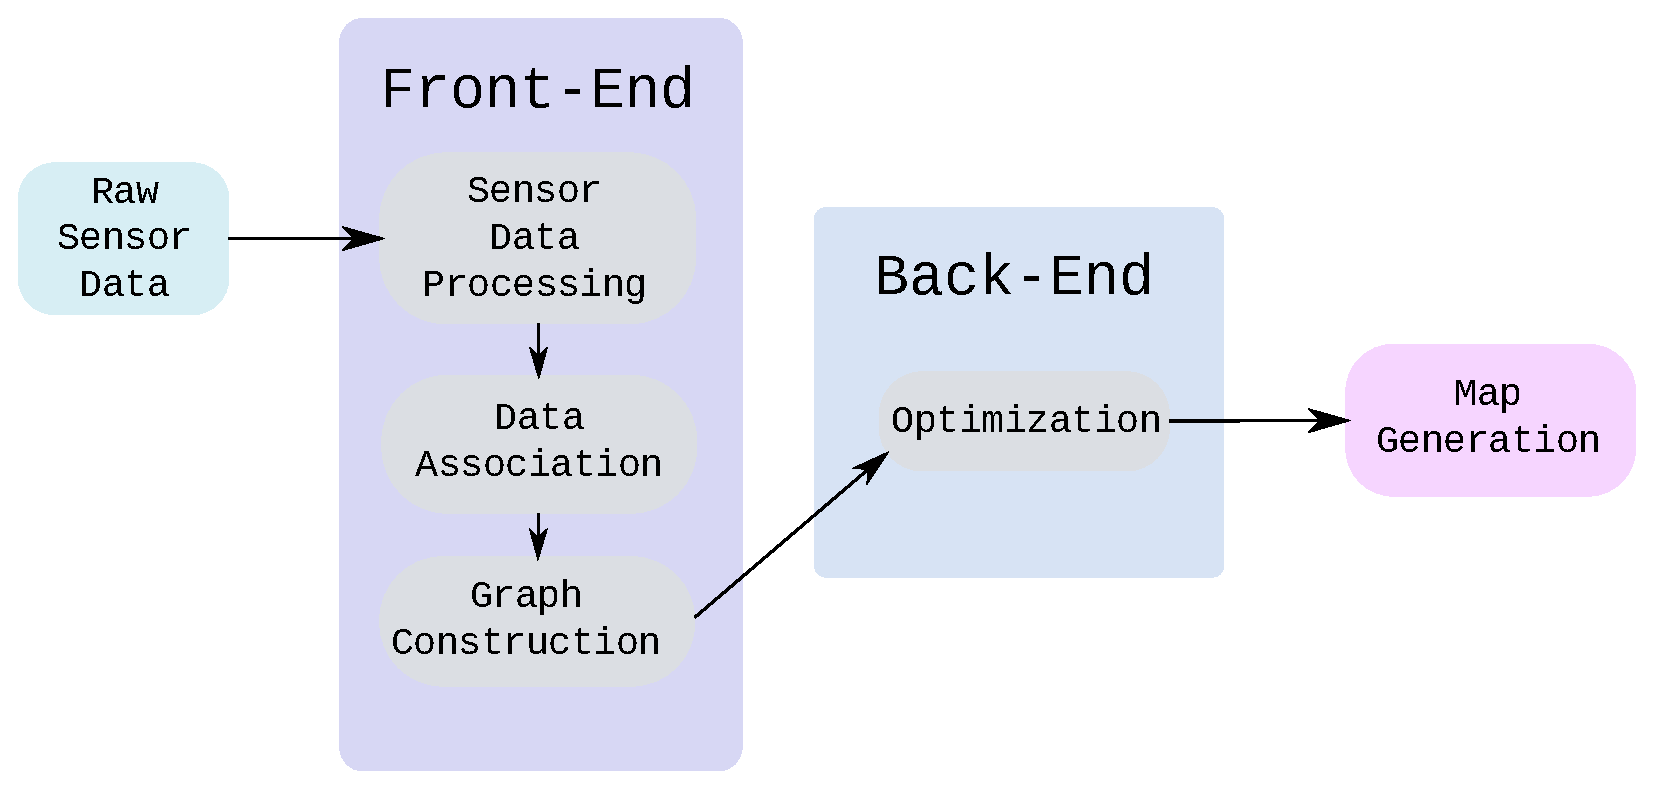
\includegraphics[width=\linewidth,natwidth=640,natheight=640]
	{figures/drawings/slam_frontend_backend.eps}
	\caption{\acrshort{slam} Framework}
	\label{fig:slam_frontend_backend}
\end{figure}


The problem that we try to tackle in this paper, in fact,
does not involve robots, instead 
\textit{pedestrians} in an indoor environment. 
This make
the \acrshort{slam} problem slightly different than mobile robotics problem.
Thus, we need to make several distinctions:

\newpage

\begin{itemize}
	\item \textbf{M}apping: A robot has the ability to explore the
	environment in such a dense way that it can create the occupancy
	grid maps and save features like unique landmarks. In pedestrian
	case, this density is not possible due to the limitations of the sensors in an average smartphone. 
	The maps created by smartphone using \acrshort{slam}
	have less resolution and topographically simpler. However, 
	this is still valuable information for smartphone user
	oriented positioning and navigation applications where 2-3 meters
	accuracy is enough. Our goal is to find a way to represent
	smartphone generated maps with the abstracted fashion. The
	candidate we choose for this purpose is \textit{pose}
	\textit{graphs}, which we will
	be explaining in section-\ref{graph_slam}.
	
	
	\item \textbf{L}ocalization: In terms of finding the accurate
	position, odometry data is much
	more precise in robots because the smartphone lacks such quality
	\acrshort{imu}s and encoders so the drifts caused 
	by motion sensors are worse in
	the smartphone. The other and critical issue is that we don't have
	the capability to recognize revisited places through feature
	extraction of landmarks. Robots are equipped with the sensors
	(e.g., RGB-D cameras, laser scanners or radars) that can provide
	high precision (2D or 3D) range and/or bearing information 
	of the landmarks. This does not only provide place recognition
	capability but also produces location information relative to the
	landmarks. If the landmark position is accurate enough, this
	information can be converted to an absolute location. 
	With the smartphone, you have the range only
	observations that one can exploit by collecting 
	\acrshort{rssi}, which is a 1D
	measurement. To get the 2D or 3D coordinate
	position, triangulation calculation is needed by measuring
	\acrshort{rssi} from at least 2 or 3 access points. Still, this \acrshort{rssi}
	triangulation methods suffer from multi-path or shadowing effect,
	which is widely known issue in \acrshort{rssi} based localization
	technologies. The other possibility is to use the mono-camera in
	smartphones but we will not be discussing in this paper.
	Since getting location information through landmark
	observations is trivial, we need to express these revisited place
	in the \acrshort{slam} concept. We achieve this need with
	\textit{fingerprint} method.
	With this method, we constantly compare the current observation
	with the fingerprint history, except we produce an error
	function that informs the optimizer how drifted we are at the
	current position. This fingerprint information can be gathered
	from \acrshort{rssi} or magnetic field measurements. 
	We will discuss this (loop closure) error
	functions in the following part of this section.
	
	\item \textbf{S}imultaneous: The difficulty of the \acrshort{slam} problem lies
	in this 'S' part, which is to generate the map during the
	localization. Two types of concurrency form are offered in the
	literature; i.e., online \acrshort{slam} in
	which the interest is in probability $p(x_{t},m|z_{1:t},u_{1:t})$
	of the current pose and full \acrshort{slam} in which interest is in probability 
	$p(x_{1:t},m|z_{1:t},u_{1:t})$ of the all the
	poses. In our case, we will be proceeding with the full \acrshort{slam}. For
	further information about general \acrshort{slam} problem, I refer readers to
	\cite{Thrun1999}.
\end{itemize}


\subsection{Graph SLAM} \label{graph_slam}

\acrshort{slam} can be modeled with the graphs in which nodes represent poses and
edges present dependencies or constraints between nodes.
\textit{\acrfull{dbg}} are suitable for comprehensive representation
and better understanding.
In \acrshort{dbg}, there exist two kinds of property; i.e.,
\textit{observable} nodes and
\textit{unobservable} nodes. Observable nodes contain the estimation of 
the pose state and of the landmark observation. However, one can never
know the real positions of the pose and of the landmarks, which are
unobservable nodes. In Figure-\ref{fig:slam_bayesian_graph}, dark
nodes are the observable node and white nodes are the unobservable
nodes:


\begin{figure}[H]
	\centering
	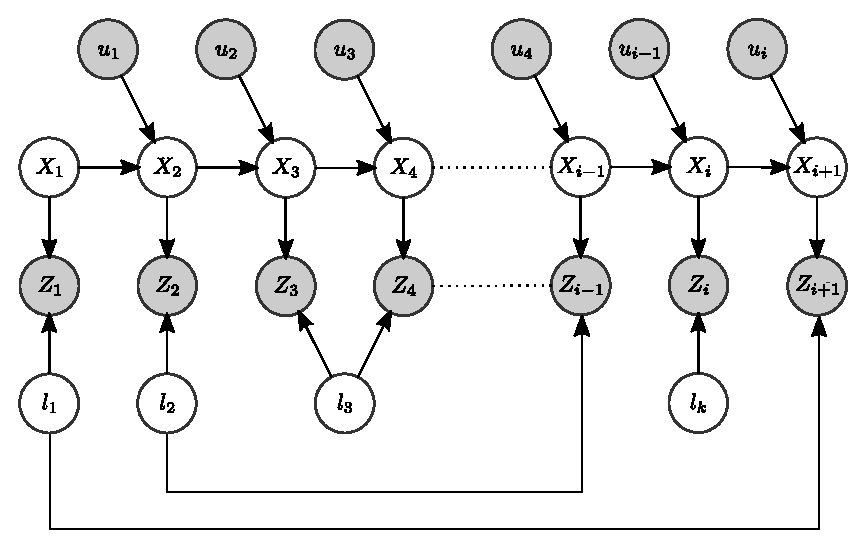
\includegraphics[width=\linewidth]
	{figures/drawings/slam_bayesian_graph_v2.eps}
	\caption{Dynamic Bayesian Graph}
	\label{fig:slam_bayesian_graph}
\end{figure}

IMPROVE below!
\begin{itemize}
	\item True pose states: $X_{1:i+1}$\footnote{True pose
		state can mean real world positions $(x_i,y_i,z_i)$, 
		real wold heading $\theta_i$ or both. 
		Similarly, true landmark state can have similar properties,
		$(l_i^x,l_i^y,l_i^z)$ and $l_i^{\theta}$.}
	
	\item Estimated pose states and landmark states:
	$Z_{1:i+1}$\footnote{Based on the model, we can estimate
		positions and heading 
		$(\widehat{x_i}, \widehat{y_i}, \widehat{z_i},
		\widehat{\theta_i})$, and landmark positions 
		$(\widehat{l_i^x},\widehat{l_i^y}, 
		\widehat{l_i^z},\widehat{l_i^{\theta})}$ 
		or both.} 
	
	\item True landmark states: $l_{1:k}$
	
	\item Estimated control actions: $u_{1:i}$\footnote{Estimated
		control actions can be a displacement vector 
		$(\Delta x, \Delta y, \Delta \theta)$.}
\end{itemize}

Notice in Figure-\ref{fig:slam_bayesian_graph} 
that $l_{1}$ is observed both in $X_{1}$ and $X_{i+1}$ 
pose states. This means that those two poses are the revisited place.
Same rule applies for the $l_{2}$ and $l_{3}$.

Another graph representation of the \acrshort{slam} is called
\textit{Factor} \textit{Graph}, which
is a compressed version of \acrshort{dbg} where pose states have relations
via undirected edges in a much simpler way. 
This type of graph is also called bipartite
undirected graphs. Since we don't distinguish true and estimated pose
in Factor Graph, we will refer as $X_{1:i+1}$ pose nodes from now on.
In Figure-\ref{fig:slam_factor_graph}, pose nodes are connected two types
of edges; i.e., red edges, representing the odometry constraints 
and blue edges, representing the landmark constraints, 
which are also called \textit{loop closures} constraints.


\begin{figure}[H]
	\centering
	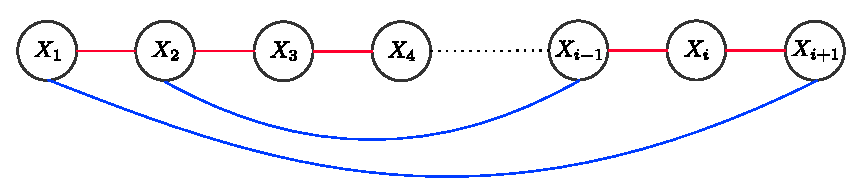
\includegraphics[width=\linewidth,natwidth=640,natheight=640]
	{figures/drawings/slam_factor_graph.eps}
	\caption{\acrshort{slam} Factor Graph}
	\label{fig:slam_factor_graph}
\end{figure}

In the case of a smartphone, pose nodes relates to step events. 
In addition, red edges
connect two successive steps via \acrshort{pdr} information and blue edges
connect two revisited pose nodes that are proposed by \acrshort{rssi} or 
magnetic field
observation. Further details about how we create the blue edges 
will be discussed in section-\ref{graph_slam_setup}.

\begin{figure}[H]
	\centering
	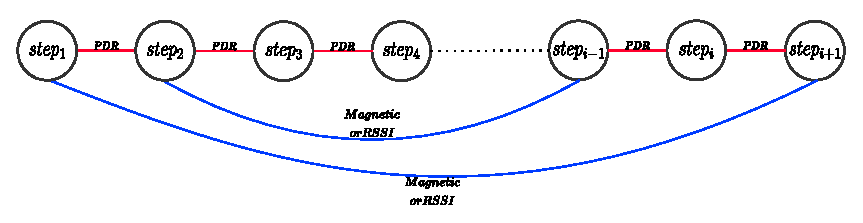
\includegraphics[width=\linewidth,natwidth=640,natheight=640]
	{figures/drawings/slam_factor_graph_indoor_case.eps}
	\caption{\acrshort{slam} Factor Graph (Indoor Scenario)}
	\label{fig:slam_factor_graph_indoor_case}
\end{figure}

\subsection{Simulation Environment for Graph \acrshort{slam}} \label{sim_graph_slam}

The graph representation of the \acrshort{slam} problem provides a sufficient
modeling; however, 
the intuition gets much clearer when we combine 
with the walking path visualization. For this reason, 
we create a simulation
environment in Matlab for our smartphone \acrshort{slam} purposes. 
Initially, a ground truth walking path with the 125 steps and 5 access
points\footnote{In the simulation environment, we gathered landmark
	constraints only from \acrshort{rssi} measurements. We did not implement
	magnetic field fingerprint method 
	at this stage, since we only used this simulation
	environment for testing the robustness of \acrshort{slam} algorithm in terms of
	smartphone application.} 
as landmarks are created. 
The starting position for the walking is $(x_0,y_0)=(0m,0m)$ 
and the ending
position is $(x_{125},y_{125})=(25m,0m)$ as it can be see in 
Figure-\ref{fig:lc_ground_truth}. We also assume that at least 
one \acrshort{rssi} measurement
from each access point is available and is stored at each step. 

\begin{figure}[H]
	\includegraphics[width=\linewidth,natwidth=640,natheight=640]
	{figures/lc_ground_truth.jpg}
	\centering
	\caption{Ground Truth in the Simulation Environment}
	\label{fig:lc_ground_truth}
\end{figure}

Then, noise is introduced to the system to represent the
\textit{drifting}
\textit{effect} of the \acrshort{imu} sensors. In Figure-\ref{fig:lc_noisy_path}, the walking
path starts from the same position but it gets drifted by
noisy step length and step heading measurement and it ends at
$(x_{125},y_{125}) = (31.6m,6.1m)$, which $8.9m$ away from its
real position. The biggest motivation behind the \acrshort{slam} is not only to
correct the current localization error but to correct the
whole walking path by keeping the topology of the route as close as
possible to the ground truth. Note that, we still hold \acrshort{rssi}
measurements from each access point in every step. Thus, we can
build the \textit{loop closures} for the revisit locations.

\begin{figure}[H]
	\centering
	\includegraphics[width=\linewidth,natwidth=640,natheight=640]
	{figures/lc_noisy_path.jpg}
	\caption{Noisy Path in the Simulation Environment}
	\label{fig:lc_noisy_path}
\end{figure}

As we can see in the ground truth path, 
the starting point is revisited at the $100^{th}$ step 
after walking a square shaped path. After this moment each step starts
to relate to its own revisited location 
since it is the same walking route after $100^{th}$ step. 
In Figure-\ref{fig:lc_true_positives}, the loop closures
are represented with the red lines. 

\begin{figure}[H]
	\centering
	\includegraphics[width=\linewidth,natwidth=640,natheight=640]
	{figures/lc_true_positives.jpg}
	\caption{True Positives Loop Closures in the Simulation Environment}
	\label{fig:lc_true_positives}
\end{figure}


\subsection{Graph SLAM Formulation} \label{graph_slam_formulation}

For our mapping purposes, it is sufficient that we have 2D
cartesian plane and represent this plane with the state vector
$\boldsymbol{x}=(x,y)^{\intercal}$. 
The motion model that we are going to build requires an assumption,
which will help us to leverage efficient statistical methods. The
assumption is that successive poses and landmark poses are 
\textit{normally distributed random variables} 
with variance $\Sigma_{i}$ and $\Lambda{ij}$, respectively. $x_{i+1}$
represent the next pose after $x_{i}$.


\begin{equation}
x_{i+1} \sim \mathcal{N} (f(x_{i},u_{i}), \Sigma_{i})
\label{eq:motion_model}
\end{equation}

$x_{j}$ represents the current pose that has loop closure relationship
with $x_{i}$ pose that is visited previously. $u_{i}$ and $u_{ij}$ are
the motion control actions as we also discussed earlier.

\begin{equation}
x_{j} \sim \mathcal{N} (f(x_{i},u_{ij}), \Lambda{ij})
\label{eq:loop_closure_model}
\end{equation}

These motion models tell us that there exist pose states 
that are normally distributed.
Therefore, we aim to find such a state configuration
of the poses that we get the most likely, in technical words,
\textit{maximum a posteriori} and 
the probabilistic representation is as
follows: 

$P(X|U)$ is the conditional
probability, which represents the probability distribution of the pose
states $X$ given the control actions $U$.
That being said, we can now use the likelihood
function $P(X|U)$ to calculate 
the most likely state configuration $X^*$ as map information. 

\begin{equation}
X^{*} = \argmax_X P(X|U)
\label{eq:generic_arg_max}
\end{equation}

Then, we elaborate the probability distribution by splitting into two
using motion models, i.e., odometry and loop closures. 
In addition to splitting, we
can define the joint probability of each pose by the product rule so
that the estimation for the state of each pose contributes the
overall likelihood.

\begin{equation}
P(X|U) \propto  
\underbrace{\prod_{i} P(x_{i+1}|x_{i},u_{i})}_{\text{Odometry Constraints}} 
\cdot 
\underbrace{\prod_{ij} P(x_{j}|x_{i},u_{ij})}_{\text{Loop Closure Constraints}}
\label{eq:probability_product}
\end{equation}

Now, we transform our problem to make it more computational friendly
since calculating products is inefficient. However, derivation from
equation \ref{eq:probability_product} to \ref{eq:sum_of_squared_errors}
is not provided in this paper and I want to refer readers to
\cite{Sunderhauf2012a}. The author 
explained the derivation in detail in his Ph.D.
thesis. To
calculate the maximum of the joint probability of our problem, we perform
the \textit{error minimization} approach so that 
we don't have to predict
the state randomly. The idea is to minimize
the difference between model estimations $\widehat{x_i}$ and
state observations $x_i$. 
With this approach, one can \textit{constrain} the
state estimation from less likely ones. Then, maximum likelihood
can be reached with an iterative error minimizing method, e.g., Least
Squares method, which we will be discussing further in section-\ref{lsq}.

As we have two motion models, we have two
parts in equation \ref{eq:sum_of_squared_errors} as well. 
For the odometry, the
estimation for the next pose $\widehat{x_{i+1}}$ will be calculated by
the model function $f(x_i,u_i)$.
Same logic applies
for the loop closure, except the loop closures might not necessarily 
represent the
consecutive steps. That is the reason we have $(i,j)$
pose pairs indexing.

\begin{equation}
X^{*} = \argmin_X = 
\underbrace{\sum_{i} \Vert f(x_{i},u_{i}) - x_{i+1}
	\Vert_{\Sigma_{i}}^{2}}_{\text{Odometry Constraints}}
+ 
\underbrace{\sum_{ij} \Vert f(x_{i},u_{ij}) - x_{j}
	\Vert_{\Lambda{ij}}^{2}}_{\text{Loop Closure Constraints}}
\label{eq:sum_of_squared_errors}
\end{equation}

Next step is to minimize the error function that we described using
Least Squares optimization method.

\subsection{Least Squares} \label{lsq}

As we discussed in the previous, error minimization
operation is required to get the maximum likelihood. To do so,
we search the most
likely state configuration as close as possible to its ground
truth. Before
plugging the least square part into our \acrshort{slam} problem, 
we explain how this method works.

Least squares problem is a non-linear optimization problem.
The goal is to find interesting points, such as local/global
maximum or local/global minimum, on the \textit{objective}
\textit{function}. Due to the
non-linearity, one can only approximate by
generating a quadratic model of the objective function and iterate
through the interest points using \textit{Newton's} methods. 
For example,
the interest point in
Figure-\ref{fig:lsq_multivariable_function_example} is at the local
minimum that is highlighted as a red point cloud.

\begin{figure}[H]
	\centering
	\includegraphics[width=\linewidth,natwidth=640,natheight=640]
	{figures/lsq_multivariable_function_example.jpg}
	\caption{Local Minimum at a Quadratic Function}
	\label{fig:lsq_multivariable_function_example}
\end{figure}


In literature,
there are many versions of Newton's method 
and they all try to find the
maximum/minimum points in the most efficient way.
\acrfull{lm} 
method, which solves this optimization problem
with the gradient descent approach with the help of 
the approximated Hessian function, is one of them and we will be using
it in our \acrshort{slam} algorithm.

Suppose that we have a model function $g(x;a)$. However,
we don't know what the $x=(x_1,x_2)$ coefficients (also called
\textit{optimization} \textit{parameters}) are and we can only
plug $a$, which is the \textit{independent} variable, into the
\textit{model} $S$ to see
how the output of the model changes given the independent variable. 

\begin{figure}[H]
	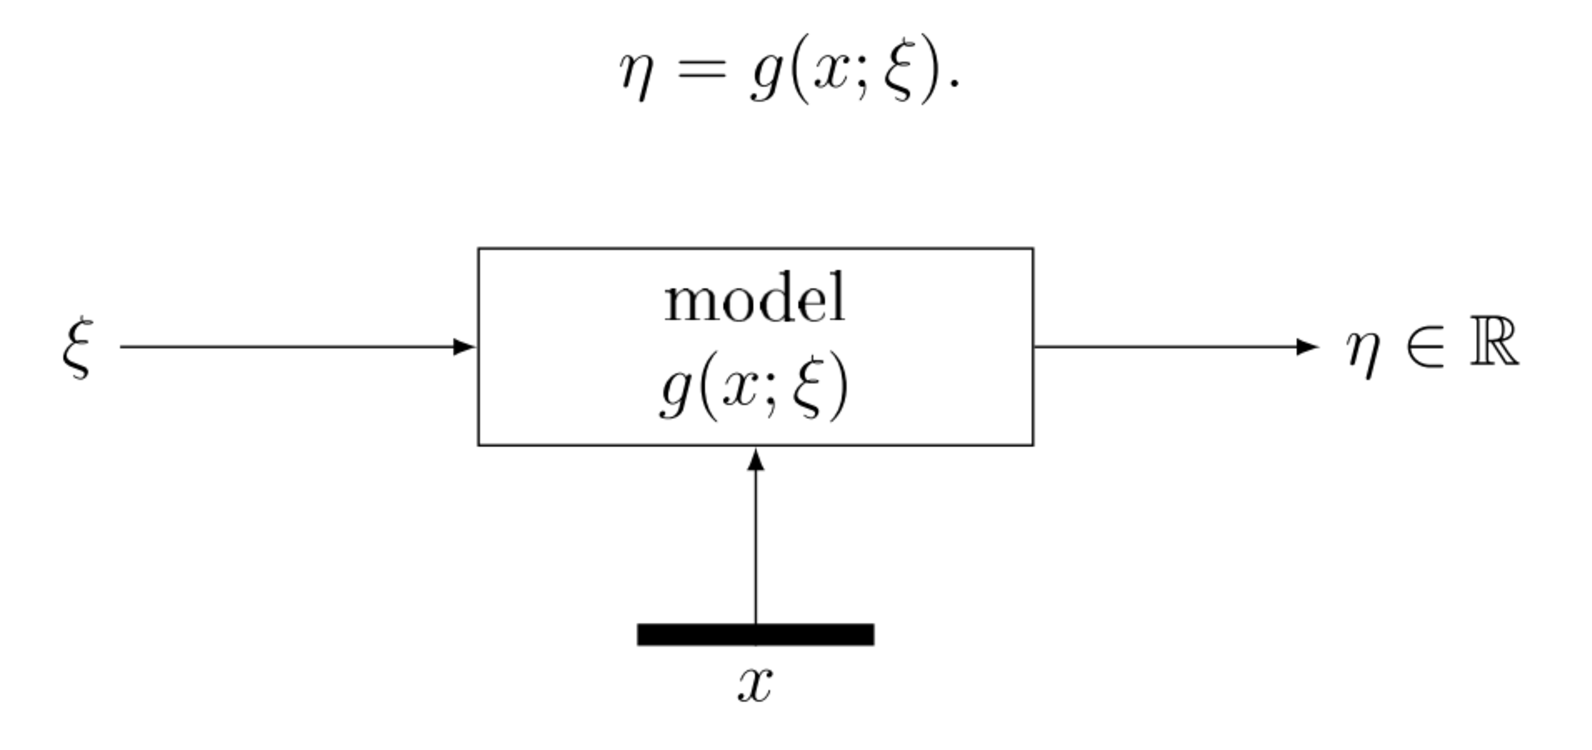
\includegraphics[width=0.8\linewidth,natwidth=640,natheight=640]
	{figures/drawings/lsq_model.jpg}
	\centering
	\caption{Least Square Model}
	\label{fig:lsq_model}
\end{figure}



\begin{gather}
\xi = a \text{ (independent variable)} \in \R \\
\eta = S \text{ (dependent variable)} \in \R
\label{eq:lsq_model_variables}
\end{gather}

\begin{equation}
S = g(x;a) := x_1 + x_2a \quad 
\text{where} \quad 
x=(x_1,x_2) \in \R^2
\label{eq}
\end{equation}


To see this effect, 
we draw a graph that is shown in
Figure-\ref{fig:lsq_curve_fit_measurements}.

\begin{figure}[H]
	\centering
	\includegraphics[width=\linewidth,natwidth=640,natheight=640]
	{figures/lsq_curve_fit_measurements_v2.jpg}
	\caption{Least Squares Measurements}
	\label{fig:lsq_curve_fit_measurements}
\end{figure}


Our goal is now to find a linear function, which will fit this
dataset. This is a typical least squares curve fitting problem, which
we construct a \textit{residuals} function $r_i(x)$ by providing
difference values between model estimation $g(x;a_i)$ and dependent
variable $S_i$. In this case, the dependent variable 
represent the real world
measurements and the residuals function represents the error between the estimated value and measurement value. 

\begin{equation}
r_i(x) := g(x;a_i) - S_i \qquad \text{ for }  i = 1,\dots,m.
\label{eq:}
\end{equation}

Then, residuals function is squared to magnify larger error effect. 

\begin{equation}
\begin{aligned}
f(x) & := \sum_{i=1}^{m} \vert r_i(x) \vert^2 = 
\sum_{i=1}^{m} \vert g(x;a_i) - S_i \vert^2 =
\sum_{i=1}^{m} (g(x;a_i) - S_i)^2 \\
\label{eq}
\end{aligned}
\end{equation}

Now, we use the sum of squared error function to calculate the most likely
configuration that can minimize the errors:

\begin{equation}
X^* = \argmin_x F(x) = \argmin_x \frac{1}{2} f(x)^\intercal f(x) = 
\sum_{i=1}^{m} (g(x;a_i) - S_i)^2, 
\quad x \in \R^2
\label{eq}
\end{equation}

At this point, the objective function is ready to be handed over to 
\acrshort{lm} method. The method will try to find the
\textit{optimal} solution $X^*$ by minimizing the objective function.

\begin{equation}
\text{Minimize} \quad \sum_{i=1}^{m} (g(x;a_i) - S_i)^2, 
\quad x \in \R^2
\label{eq}
\end{equation}

To help our understanding, the objective function is drawn in
Figure-\ref{fig:lsq_sum_of_squared_error_function}.
As we can see, the based on the given $x=(x_1,x_2)$ values, 
the objective
function $F(x)$ behave as follows:

\begin{figure}[H]
	\centering
	\includegraphics[width=\linewidth,natwidth=640,natheight=640]
	{figures/lsq_sum_of_squared_error_function_v2.jpg}
	\caption{Local Minimum at Sum of Squared Error Function}
	\label{fig:lsq_sum_of_squared_error_function}
\end{figure}

The initial guess for the optimization parameters at $x=(4,4)$, which
is highlighted as a blue color point cloud and 
the local minimum point, which is the interest point of ours, 
is highlighted with the red cloud. \acrshort{lm} method uses its gradient
descent strategy to travel to the nearest local minimum. As we can see
that the descent is successfully performed and the optimization
operation results in the $x=(1.9,2.1)$. 


If we now place the optimization variables into our model function, we
get the $g(x;a)=1.9+2.1a$ and a fitted line based on the given
dataset in
Figure-\ref{fig:lsq_curve_fit_operation}.

\begin{figure}[H]
	\centering
	\includegraphics[width=\linewidth,natwidth=640,natheight=640]
	{figures/lsq_curve_fit_operation_v2.jpg}
	\caption{Least Squares Curve Fitting Operation}
	\label{fig:lsq_curve_fit_operation}
\end{figure}

Keep mind that there are
crucial factors whether \acrshort{lm} will descent the local minimum to the
interest point or not:
\begin{itemize}
  \item \textit{outliers} in the dataset,
  \item good \textit{initial point guess}. 
\end{itemize}

If these two criteria do not meet, \acrshort{lm} might converge to the
another local minimum or might not even converge to
an optimal solution. It is important that we provide a good initial
guess and minimum amount of outliers into any gradient descent
optimization algorithm. Otherwise, we will not be able to converge to
a local minimum that we are interested in since we will be stuck at
another local minimum point. 
Not being able to find an optimal solution 
in \acrshort{slam} context will result in 
an estimated state configuration is largely
different from the ground truth.


\subsection{Graph SLAM Setup for Smartphone} \label{graph_slam_setup}

So far, we discussed how the general Graph \acrshort{slam} problem is
formulated. In this section, I am going to reformulate the Graph \acrshort{slam}
for the smartphone scenario. We already mentioned that odometry in
robotics relates to step event in the smartphone. Therefore, we replace
the odometry motion model with the \acrshort{pdr} motion model.
In this model, each step will have a state vector with 
$\boldsymbol{x}=(x,y)$, represents the 2D position coordinates.
We don't include heading information into the
objective function that is used for optimization of the walking path
for our experiments. 

The distinct separation for the smartphone \acrshort{slam} is that landmark
observations and its contribution to the optimization process. 
Usually, mobile robots are equipped 
with camera sensors and/or laser sensor.
They provide 3D or 2D position results
relative to the observed landmark, which easily be converted to the
global coordinate system if the orientation of the robot is known. As
we mentioned earlier, this is not possible with the \acrshort{rssi} based
measurements as they only provide 1D measurement. Moreover, 
generating 2D
position information with triangulation techniques does not provide
accurate results. Therefore, we need to come up with a way to
recognize the revisited places without using \acrshort{rssi} positioning
capabilities. In the end, landmark observations are just loop closures
constraints that help the optimization algorithm to converge to 
the minimum. 
If we find a way to create an error
model function without using positioning algorithm, the
optimization algorithm will still try to converge the minimum since
the loop closure constraints behave like a \textit{penalization}
\textit{factor}. For a
now, we replace the 
$f(x_{i},u_{ij}) - x_{j}$ with our error function model $e_{ij}^{LC}$,
which we will explain in detail soon in this section. 

By following
previously mentioned changes, we transform the \acrshort{slam} problem into
equation-\ref{eq:smartphone_slam_formulation}.

\begin{equation}
\boldsymbol{X}^{*} = \argmin_{\boldsymbol{X}} = 
\underbrace{\sum_{i} \Vert f(\boldsymbol{x}_{i},u_{i}) -
	\boldsymbol{x}_{i+1}
	\Vert_{\Sigma_{i}}^{2}}_{\text{PDR Constraints}}
+ 
\underbrace{\sum_{ij} \Vert e_{LC}(\boldsymbol{x}_{ij})
	\Vert_{\Lambda{ij}}^{2}}_{\text{Loop Closure Constraints}}
\label{eq:smartphone_slam_formulation}
\end{equation}

To elaborate how we calculate the error function $e_{PDR}(x)$ 
based on \acrshort{pdr} constraints, the following equation is provided. 

\begin{equation} 
f_{PDR}(\boldsymbol{x}) = e_{PDR}(\boldsymbol{x}) = 
\begin{pmatrix}
f(\boldsymbol{x}_0,u_0)-\boldsymbol{z}_1 \\
f(\boldsymbol{x}_1,u_1)-\boldsymbol{z}_2 \\
\vdots \\
f(\boldsymbol{x}_{i-1},u_{i-1})-\boldsymbol{z}_i \\
\end{pmatrix}
\label{eq}
\end{equation}

The
error for each state is defined by a difference value between a model
estimation $f(\boldsymbol{x}_0,u_0)$ and a measurement
$\boldsymbol{z}$. The model
estimation produces an estimated state vector
$\boldsymbol{x}=(\Delta x_i, \Delta y_i)$. On the
other hand, the \acrshort{pdr} step detection algorithm produces a measured step
length and a heading information where combine them into a state
vector form 
$\boldsymbol{z}=
( \Delta \widehat{x_n},
\Delta \widehat{y_n})$


Notice how we create loop closures in
Figure-\ref{fig:lc_true_positives}. Due to the \acrshort{imu}
caused drift issue, the walking path results in such a shape. Thanks to
having one \acrshort{rssi} measurement from each access point in each step in the
simulation environment, we are able to recognize revisited places,
(e.g., step 0 and step 100, step 1 and step 101, so on) with
the following dissimilarity equation:

\begin{equation}
dis(RSSI_{i},RSSI_{j}) = \sqrt{\sum_{k=1}^{M} 
	\dfrac{\Vert (RSSI_{i}^{(k)} - RSSI_{j}^{(k)}) \Vert }{M}} 
\label{eq:rssi_dissimilarity_function}
\end{equation}

The dissimilarity function $dis(RSSI_k,RSSI_q)$ is simply a normalized
euclidian distance that is calculated between two \acrshort{rssi} measurement
vectors composed of surrounding access points. Note that one \acrshort{rssi}
vector is measured at $i^{th}$ step and the other one is at the
$j^{th}$ step. 

Then, if the dissimilarity
value is less the threshold that we empirically defined, we count it
$i$ and $j$ steps as a loop closure. In the simulation environment, we
take the dissimilarity threshold as 1 dBm. However, keep in mind that
the threshold value will be different when we perform \acrshort{slam} with real
measurement. 

\begin{gather}
f_{LC}(\boldsymbol{x}_{ij}) = 
e_{LC}(\boldsymbol{x}_{ij}) = 
e_{RSSI}(\boldsymbol{x}_{ij}) 
= d(i,j) = \sqrt{(x_i-x_j)^2+(y_i-y_j)^2}
\label{eq:}
\end{gather}

Next step is to form an error model $e_{RSSI}(.)$ 
for the loop closures in a way that
we can place into the objective function of our smartphone 
\acrshort{slam} optimization problem. We again remind you that loop closures in
Figure-\ref{fig:lc_true_positives} are useful to generate this error
model. The loop closure event says that step 0 and step 100 are in
fact the same place due to the similarity of their \acrshort{rssi} measurement.
By following this logic, we can also say that larger the euclidian
distance between these two step, greater the error value should be.
As a result, the loop closure will have 
more penalization effect during
optimization operation. In the end, we expect from \acrshort{lm} method to
minimize the loop closure related error function. 
In addition to this loop closure related
error function, we have the motion model error function in the
same objective function as well. 
When these two error model functions are
provided to the optimizer, \acrshort{lm} will try to 
come up with such a 
state configuration that steps having loop closures constraints 
will be as close as possible.
At the same time, the optimizer will have to keep the topological
shape intact as we have \acrshort{pdr} related constraints in
the equation.

Finally, we present the objective function of our smartphone \acrshort{slam}
problem with the following: 

\begin{equation}
F(\boldsymbol{x}) = \sum_{i=1}^{m} e^{\intercal}_{PDR}(x)
\Sigma_{i} e_{PDR}(x) + 
\sum_{(i,j)\in C} \Lambda_{ij} e_{LC}(\boldsymbol{x}_{ij})
\label{eq}
\end{equation}

The goal is to find a state configuration that minimizes the sum of
squared errors:

\begin{equation}
\boldsymbol{X}^* = \argmin_{\boldsymbol{x}} F(\boldsymbol{x})
\label{eq:}
\end{equation}

In our simulation experiments, we keep motion model variance
$\Sigma_i$ as an identity matrix and $\Lambda$ as 1. The weighting of
the each sensor measurement will be a future work.

\begin{figure}[H]
	\centering
	\includegraphics[width=\linewidth,natwidth=640,natheight=640]
	{figures/fp_slam_results.jpg}
	\caption{An Optimal Solution Found by \acrshort{lm}}
	\label{fig:fp_slam_results}
\end{figure}

We also implement the \acrshort{slam} algorithm by utilizing \acrshort{lm} method that
is already available in Matlab Optimization Toolbox. The walking path
optimization result is presented in
Figure-\ref{fig:fp_slam_results} and 
the optimized walking path is nearly
identical to the ground truth, as we can see.

\subsection{Further Modifications on Graph SLAM Setup for Smartphone} \label{further_modification_graph_slam}

Until this section, we only convert general \acrshort{slam} problem to the
smartphone \acrshort{slam} problem by relying on the simulation environment.
Nonetheless, the assumption that has been made is not realistic when
considering the real-world data. For instance, \acrshort{rssi} measurement scans
take about 2-3 seconds to complete. By the time we received the
results, the user will be at the different positions already. Also,
not having enough frequency in the scan rate disagrees with 
the assumptions that we will have at least one measurement for each.
For \acrshort{slam} to optimize the drifted path accurately, 
true positive loop closures are required but \acrshort{rssi} are prone to
produce more \textit{false} \textit{positives}\footnote{False positive is a 
	wrong statement
	that say a particular condition or attribute exist}
	than \textit{true} \textit{positives}\footnote{True positive says the condition or the
	attribute exists and it is a
	correct statement.}.
We find out that 
the simple dissimilarity function that we created is not able to
produce enough positive. \acrshort{rssi}
requires more sophisticated algorithms to recognize the revisited
places. That is the reason we experimented magnetic field sensor
measurements to perform loop closures and compare to \acrshort{rssi}.
Moreover, we try to tackle the false positive loop closures with more
robust \acrshort{slam} algorithm.

\subsubsection{Magnetic Field Loop Closures} \label{modification_mf_lc}

In addition to \acrshort{rssi}, we can also use magnetic field distortions to
recognize the revisited place because it has unique
fingerprints indoor. By comparing current step's magnetic field with
the previous steps, we can tell if there is a
correlation or not like we do with the \acrshort{rssi}.

By following the similar principle, 
we define a dissimilarity function for magnetic field
measurements:

\begin{equation}
\begin{aligned}
dis & (MF_i, MF_j) = \\ 
& \sqrt{
	(MF_{i}^{x} - MF_{j}^{x})^2-
	(MF_{i}^{y} - MF_{j}^{y})^2-
	(MF_{i}^{z} - MF_{j}^{z})^2
} 
\end{aligned}
\label{eq:}
\end{equation}

Also, the same error model function that 
we used for the \acrshort{rssi} loop closures
applies for the MF caused loop closures. 

\begin{equation}
f_{LC}(\boldsymbol{x}_{ij}) = e_{LC}(\boldsymbol{x}_{ij}) 
= e_{MF}(\boldsymbol{x}_{ij}) =
d(i,j) = \sqrt{(x_i-x_j)^2+(y_i-y_j)^2}
\label{eq}
\end{equation}


\subsubsection{How About Some False Positive Loop Closures?} \label{false_positives}

Landmark observations in \acrshort{slam} can provide such results that
the place that is recognized as a revisited
place, in fact, is a different place. 
In Figure-\ref{fig:fp_measured_walking_path_false_pos},
blue lines represent the false loop closures. 

\begin{figure}[H]
	\centering
	\includegraphics[width=\linewidth,natwidth=640,natheight=640]
	{figures/fp_measured_walking_path_false_pos.jpg}
	\caption{False Positive Loop Closures in the Simulation Environment}
	\label{fig:fp_measured_walking_path_false_pos}
\end{figure}

Unfortunately, these erroneous
data associations have a huge impact on the optimizer's performance.
Notice in Figure-\ref{fig:fp_slam_results_false_pos} that resulting
optimized walking is unsuccessful. This problem
is known as a convergence problem in \acrshort{slam}. 
Filtering out the all outliers during the front-end is
not a realistic design choice since there will be always some
outliers in place recognition, 
which will eventually result in an false
positive. Therefore, we have to deal with these false positives in the
back-end where the optimization is performed.

\begin{figure}[H]
	\centering
	\includegraphics[width=\linewidth,natwidth=640,natheight=640]
	{figures/fp_slam_results_false_pos.jpg}
	\caption{Optimized Path Results}
	\label{fig:fp_slam_results_false_pos}
\end{figure}

The \textit{robust} \textit{back-end} for Graph \acrshort{slam} approach
\cite{Sunderhauf2012} tackles
this particular problem. The intuition behind this method is to
disable the false positive loop closures by relying on expected drift
effect. For example, we know that total drift caused by \acrshort{imu} will be
up to 2 meters by the time the first loop closure occurs 
with the given walking path route. Therefore, we can assume that false
positives loop closures that are a father than 2 meters happens to be
outliers and they need to be deactivated during optimization. 

\begin{equation}
\begin{aligned}
\boldsymbol{X}^{*}, S^* & = \argmin_{\boldsymbol{X},S} = \\
& \underbrace{\sum_{i} \Vert f(\boldsymbol{x}_{i},u_{i}) -
	\boldsymbol{x}_{i+1} 
	\Vert_{\Sigma_{i}}^{2}}_{\text{PDR Constraints}} \\ 
& + 
\underbrace{\sum_{ij} \Vert sig(s_{ij}) \cdot
	e_{LC}(\boldsymbol{x}_{ij})
	\Vert_{\Lambda{ij}}^{2}}_{\text{Switched Loop Closure Constraints}}
\\
& +
\underbrace{\sum_{ij} \Vert \gamma_{ij} - s_{ij} \Vert^2_{\Xi}}_
{\textit{Switch Prior Constraint}}
\end{aligned}
\label{eq:smartphone_slam_formulation}
\end{equation}


\begin{equation}
\text{where} \quad sig(s_{ij}):\R \rightarrow (0,1) =
\dfrac{1}{1+e^{-s_{ij}}}
\label{eq}
\end{equation}

By following this logic,
the author proposes to introduce
switch variables into the objective function. By doing so, we are able
to switch off the false positives because the switch prior constraint
part will produce larger errors comparing to 
switched loop closure constraints part. During our simulation 
experiments, we
assume that the largest drift when the first loop closure happens is
less than 5 meters. Therefore, we take $\gamma_{ij} = 5$ for all loop
closure constraints as an initial guess, which means all loop
closures are active at the beginning of the optimization process.  

\begin{figure}[H]
	\centering
	\includegraphics[width=\linewidth,natwidth=640,natheight=640]
	{figures/fp_robust_backend_slam_results.jpg}
	\caption{Robust SLAM Back-end Optimizer Results}
	\label{fig:fp_robust_slam_backend_results}
\end{figure}

By updating our \acrshort{slam} formulation, we manage to converge to the optimal
solution, which results in such an optimized path 
which is close to the ground truth, 
as we see in Figure-\ref{fig:fp_robust_slam_backend_results}.



\newpage

\section{Evaluation} \label{evaluation}

Now that we prepare our \acrshort{slam} recipe for Smartphone, it is time to
evaluate how it performs with the real-world data and I will try to
answer these two following questions in this section:

\begin{itemize}
	\item Which of sensors that used for loop closures performs better
	than the other in terms of path convergence?
	\item What is the accuracy of the converged path results?
\end{itemize}


\subsection{Device and Environment Settings} \label{device_settings}

The device that we used in our experiments is the Lenovo PB2 and
its technical summary is the following:

\begin{table}[H]
	\centering
	\caption{Test Device Properties}
	\label{table:test_device_properties}
	\renewcommand{\arraystretch}{1.5}
	\begin{tabular}{|l|c|}
		\hline
		Phone Model               &  Lenovo PB2-690M \\ \hline
		Android OS  & 6.0.1 \\ \hline
		Accelerometer             & Bosch Sensortec BMI160 \\ \hline
		Gyroscope   &  Bosch Sensortec BMI160 \\ \hline 
		Magnetometer & Asahi Kasei Microdevices AK09911 \\ \hline
	\end{tabular}
\end{table}

Overall, we collected 3 different datasets, each having different
route in $4^{th}$ floor's two office of 
the Weinholdbau Campus of TU Chemnitz, as it is given in 
Figure-\ref{fig:datasets}. The datasets' properties are the following:

\begin{itemize}
  \item \textit{Dataset} \textit{1}\footnote{\acrshort{ble} beacons 
		location are represented as blue stars on the figure.} 
	has rectangle shape route and is completed in 258
	steps by covering the same path 5 times.
      \item \textit{Dataset} \textit{2} represents a more natural walking style 
	and the route is completed in 425 steps by covering
	the same path 4 times.
      \item \textit{Dataset} \textit{3} covers a bigger region comparing to other two
	ones. The route is completed in 926 steps by covering the same
	path 3 times.
\end{itemize}


\begin{figure}[H]
	\centering
	\begin{subfigure}[b]{0.475\textwidth}
		\centering
		\includegraphics[width=\textwidth]
		{figures/reference_path_640_square_v3.png}
		\caption[]
		{{\small Dataset 1}}    
		\label{fig:dataset1}
	\end{subfigure}
	\hfill
	\begin{subfigure}[b]{0.51\textwidth}  
		\centering 
		\includegraphics[width=\textwidth]
		{figures/reference_path_640_strolling_v1.png}
		\caption[]
		{{\small Dataset 2}}    
		\label{fig:dataset2}
	\end{subfigure}
	\vskip\baselineskip
	\begin{subfigure}[b]{0.8\textwidth}  
		\centering 
		\includegraphics[width=\textwidth]
		{figures/long_straight_base_v1.png}
		\caption[]
		{{\small Dataset 3}}    
		\label{fig:dataset3}
	\end{subfigure}
	\caption[]
	{\small Collected Datasets} 
	\label{fig:datasets}
	
\end{figure}


Since any precise ground truth map information wasn't available for
the indoor environment in which 
we collected our dataset, we build it with
\acrshort{pdr} algorithm. Although \acrshort{pdr} has drift issues, it provides accurate
positioning results for a short time. 
Note that, \acrshort{pdr} algorithm that is used for the
ground truth contains accelerometer and gyroscope sensor information
for the ground truth. That's the reason we don't experience
substantial drift. However, we don't have an absolute heading
information unless the magnetometer isn't fused. Hence, we manually
oriented the initial heading so that we have a global reference frame
that we perform comparisons. 
The other issue with the ground truth is that
we don't know how much exactly the created
ground truth deviates from the real walking path. 
However, the main goal of this paper is to find out how \acrshort{slam} is
able to recover the walking path shape.


\subsection{Wi-Fi Loop Closures} \label{wifi_lc}

In the simulation environment, we assume that each step has at least
one \acrshort{rssi} measurement from its surrounding access points. This is not
a realistic assumption. The Lenovo PB2 devices provides 
1-2 seconds Wi-Fi scan period, which is 
relatively
fast Wi-Fi comparing to the other Android smartphones in
the market, but it is still not enough for assumption for 
at least one \acrshort{rssi}
measurement for each step. 

By keeping these limitations in mind, we build the dataset as follows:

\begin{itemize}
	\item Walking Path: Dataset 1
	\item \acrshort{imu} Scan Rate: 20 ms
	\item Wi-Fi Scan Rate: 1-2 ms (depends on the OS)
	\item Dissimilarity threshold: 5 dBm
	\item Temporal distance threshold\footnote{When recognizing
		revisited
		places, consecutive steps' fingerprint information is highly
		correlated with each other. Therefore, we reject loop closures
		occurred within 10 s.}: 10 s
\end{itemize}

Based on the given setup, we experience loop closures that is shown in
the Figure-\ref{fig:slam_wifi_lc}


\begin{figure}[H]
	\centering
	\begin{subfigure}[b]{0.475\textwidth}
		\centering
		\includegraphics[width=\textwidth]
		{figures/slam_wifi_lc.jpg}
		\caption[]
		{{\small Loop Closures}}    
		\label{fig:slam_wifi_lc}
	\end{subfigure}
	\hfill
	\begin{subfigure}[b]{0.475\textwidth}  
		\centering 
		\includegraphics[width=\textwidth]
		{figures/slam_wifi_optimized_path.jpg}
		\caption[]
		{{\small Optimized Path}}    
		\label{fig:slam_wifi_optimized_path}
	\end{subfigure}
	\caption[]
	{\small Dataset 1 Optimization with Wi-Fi} 
	\label{fig:square_walking_path_optimized_with_wifi}
\end{figure}


Then, we run \acrshort{lm} optimization algorithm and the resulting walking
path configuration is shown in
Figure-\ref{fig:slam_wifi_optimized_path}. Clearly, the optimal
solution is not founded due to the lack true positive loop closures.
The majority of the loop closures are false positives. Therefore, 
\acrshort{lm} algorithm does not converge.

\subsection{BLE Loop Closures} \label{ble_lc}

The other \acrshort{rssi} type measurement is collected by using 
\acrshort{ble} technology. The main difference between Wi-Fi and BLE in
terms of \acrshort{slam} is that \acrshort{ble} provides much higher scan rate, which could
meet the assumption for at least one \acrshort{rssi} measurement for each step.
However, the problem with the \acrshort{ble} is the deviation of \acrshort{rssi}
measurement, which causes many false positive loop closures. In
Figure-\ref{fig:slam_ble_lc}, the graph is almost covered by the loop
closures due to the false positives.

Dataset setup for the \acrshort{ble} is as follows:

\begin{itemize}
	\item Walking Path: Dataset 1
	\item \acrshort{imu} scan rate: 20 ms
	\item \acrshort{ble} scan rate: 200 ms
	\item Dissimilarity threshold: 1 dBm
	\item Temporal distance threshold: 10 s
\end{itemize}


\begin{figure}[H]
	\centering
	\begin{subfigure}[b]{0.475\textwidth}
		\centering
		\includegraphics[width=\textwidth]
		{figures/slam_ble_lc.jpg}
		\caption[]
		{{\small Loop Closures}}    
		\label{fig:slam_ble_lc}
	\end{subfigure}
	\hfill
	\begin{subfigure}[b]{0.475\textwidth}  
		\centering 
		\includegraphics[width=\textwidth]
		{figures/slam_ble_optimized_path.jpg}
		\caption[]
		{{\small Optimized Path}}    
		\label{fig:slam_ble_optimized_path}
	\end{subfigure}
	\caption[]
	{\small Dataset 1 Optimization with \acrshort{ble}} 
	\label{fig:square_walking_path_optimized_with_ble}
\end{figure}


With the presence of great amount of false positives, we can see that
\acrshort{lm} does not converge to the optimal solution that we seek, as we
see in Figure-\ref{fig:slam_ble_optimized_path}.


\subsection{Magnetic Loop Closures} \label{mf_lc}

The last loop closure method is the magnetic field. None of the
issues we had in \acrshort{rssi} does not appear in this case, as we can see in
Figure-\ref{fig:slam_mag_lc}. Majority of the loop closure are true
positives. The main reason for such a successful recognition of
revisited places is that we store the 3-axis local magnetic field data
based on the orientation of the device's body. If the user 
revisits any place again in future by holding the device at the
similar position and orientation, the dissimilarity function is
able to detect this behavior as a loop closure.

Magnetic field loop closure setup is as follows:

\begin{itemize}
	\item Walking Path: Dataset 1,2 and 3
	\item \acrshort{imu} scan rate: 20ms
	\item Magnetometer scan rate: 20 ms (same magnetic field value that
	is used in \acrshort{imu})
	\item Dissimilarity threshold: \SI{1}{\micro\farad}
	\item Temporal distance threshold: 10 s
\end{itemize}


\begin{figure}[H]
	\centering
	\begin{subfigure}[b]{0.475\textwidth}
		\centering
		\includegraphics[width=\textwidth]
		{figures/slam_mag_lc.jpg}
		\caption[]
		{{\small Loop Closures}}    
		\label{fig:slam_mag_lc}
	\end{subfigure}
	\hfill
	\begin{subfigure}[b]{0.475\textwidth}  
		\centering 
		\includegraphics[width=\textwidth]
		{figures/slam_mag_optimized_path.jpg}
		\caption[]
		{{\small Optimized Path}}    
		\label{fig:slam_mag_optimized_path}
	\end{subfigure}
	\caption[]
	{\small Dataset 1 Optimization
		with Magnetic Field} 
	\label{fig:square_walking_path_optimized_with_mag}
\end{figure}


The resulting optimized path by the magnetic field is shown in
Figure-\ref{fig:slam_mag_optimized_path}. \acrshort{slam} achieves to converge
to an optimal solution that is close to the ground truth.

Again with the Magnetic Field loop closures on Dataset 2, 
majority of the loop
closure are true positives as it is seen in
Figure-\ref{fig:strolling_magnetic_lc}.


\begin{figure}[H]
	\centering
	\begin{subfigure}[b]{0.475\textwidth}
		\centering
		\includegraphics[width=\textwidth]
		{figures/strolling_magnetic_lc.jpg}
		\caption[]
		{{\small Loop Closures}}    
		\label{fig:strolling_magnetic_lc}
	\end{subfigure}
	\hfill
	\begin{subfigure}[b]{0.475\textwidth}  
		\centering 
		\includegraphics[width=\textwidth]
		{figures/strolling_magnetic_optimized_path.jpg}
		\caption[]
		{{\small Optimized Path}}    
		\label{fig:strolling_magnetic_optimized_path}
	\end{subfigure}
	\caption[]
	{\small Dataset 2 Optimization  
		with Magnetic Field} 
	\label{fig:strolling_walking_path_optimized_with_mag}
\end{figure}

\newpage

In Figure-\ref{fig:strolling_magnetic_optimized_path} 
optimized path result is shown. In this dataset, we experience more
deviations from the ground truth comparing to Dataset 1. 
However, the optimizer still manages to converge to an acceptable
solution since the topology is kept mostly intact.


The third and last dataset 
that we collected expands to a bigger region by
covering more rooms and the reference path of the walking route.
Now, our algorithm faces the challenge against converging 
to an optimal path. Remember that our robust \acrshort{slam} back-end deactivates
the false positive loop closures because we assume that outliers could
only occur when the distance between two loop closure point is too
large. 
However, the assumption fails when we detect the 
false positive loop closures between room 463 and room 460, as it is
shown in Figure-\ref{fig:long_straight_lc}.
At this point, the
algorithm cannot reject these false positives 
because our threshold for
rejecting false positive is 10 meters. Therefore, the resulting path
is at these poses are distorted between these two rooms, as we can see
in Figure-\ref{fig:long_straight_optimized_path}. 
If we, on the other hand, lowered the
threshold to 4 meters, we could reject them. By doing so, we would
also be rejecting most of the true positives as well and we would be
able to converge at all. 
This is the
trade-off that the algorithm faces.

\begin{figure}[H]
	\centering
	\begin{subfigure}[b]{0.475\textwidth}
		\centering
		\includegraphics[width=\textwidth]
		{figures/long_straight_lc.jpg}
		\caption[]
		{{\small Loop Closures}}    
		\label{fig:long_straight_lc}
	\end{subfigure}
	\hfill %\vskip\baselineskip
	\begin{subfigure}[b]{0.475\textwidth}  
		\centering 
		\includegraphics[width=\textwidth]
		{figures/long_straight_optimized_path.jpg}
		\caption[]
		{{\small Optimized Path}}    
		\label{fig:long_straight_optimized_path}
	\end{subfigure}
	\caption[]
	{\small Dataset 3 Optimization with Magnetic Field} 
	\label{fig:long_straight_walking_path}
\end{figure}


\subsection{Root Mean Square Error Evaluation} \label{sec:rmse}

Finally, we provide the statistical error evaluation and
the method, selected for the evaluation, is
the \textit{\acrfull{rmse}}. This method measures the 
average deviation of the estimated positions from the
ground truth positions. We only consider 2D in our experiments:

\begin{equation}
RMSE = \sqrt{
	\dfrac{1}{n} \sum_{i=1}^{n} 
	(\boldsymbol{x}_{x,y}^{(i)} - \widehat{\boldsymbol{x}_{x,y}^{(i)}}
	)^2
}
\label{eq:}
\end{equation}

where $\boldsymbol{x}_{x,y}^{(i)} = (x_i,y_i)$ are the ground truth
positions and $\widehat{\boldsymbol{x}_{x,y}^{(i)}} = (\widehat{x_i},
\widehat{y_i})$ are the estimated positions. Here is the comparison
across all datasets that we collected so far:


\begin{table}[H]
	\centering
	\caption{\acrshort{rmse} Comparison Between Datasets}
	\label{my-label}
	\renewcommand{\arraystretch}{1.5}
	\begin{tabular}{llcc}
		\hline
		Dataset & Loop Closure Type & RSME (x,y) & Convergence \\ \hline
		1 & \acrshort{ble} & (2.9278,3.8333) & No \\
		1 & Wi-Fi & (0.6863,2.8734) & No \\
		1 & Magnetic Field & (0.6835,0.6835) & Yes \\ \hline 
		2 & Magnetic Field & (2.1992,2.1173) & Yes \\  \hline
		3 & Magnetic Field & (5.4413, 3.2115) & No \\ \hline
	\end{tabular}
\end{table}



\newpage


\section{Conclusion} \label{conclusion}

In this research paper, we studied \acrshort{slam} problem to solve 
the indoor mapping problem. After stating our motivation for the
paper, we shortly described how \acrshort{pdr} algorithm works and identify
its limitations. Since the goal of the paper is to recover \acrshort{pdr}'s
walking path drifts by the Graph \acrshort{slam}, we explained the general
formulation. Then, we convert this formulation to such a form that one
can utilize it with the smartphone. As a result of this study, we 
gained the following insights:

\begin{itemize}
	\item Graph \acrshort{slam} has a great potential to be a
	  \textit{recovery} \textit{mechanism}
	against the drifted walking path caused by the smartphone's \acrshort{imu}. 
	\item A general Graph \acrshort{slam} formulation fails to converge to the
	optimal solution with the presence of false loop closures.
	Therefore, more \textit{robust} version of \acrshort{slam} is required to deal with
	the outliers.
      \item \textit{Magnetic} \textit{field} outperforms both Wi-Fi and \acrshort{ble} in terms of
	loop closure detection. However, the map builder individuals must
	walk by following such routes that they constantly revisit the
	place as frequent as possible. \acrshort{slam}
\end{itemize}



\newpage

\section{Bibliography}




%deleting auto-generated reference title
\renewcommand\refname{\vskip -1cm} 


\nocite{*}


\bibliographystyle{alpha}
\bibliography{ref}



\end{document}



